\documentclass[a4 paper]{article}

% Set target color model to RGB
\usepackage{amsmath}
\usepackage{tikz}
\usepackage[ruled,vlined]{algorithm2e}
\usepackage{graphicx}
\usepackage{mathrsfs}
\usepackage{amssymb}
\usepackage{titlesec}
\usepackage{booktabs}
\usepackage{array}
\usepackage{geometry}
\usepackage{multirow}
\usepackage{tabularx}
\usepackage{wrapfig}
\usepackage{natbib}
\usepackage{tocloft}
\usepackage{subcaption}

\newcommand{\ra}[1]{\renewcommand{\arraystretch}{#1}}

\newcommand{\project}[4]{
   \pagestyle{myheadings}
   \thispagestyle{plain}
   \newpage
   \setcounter{page}{1}
   \noindent
   \begin{center}
   \framebox{
      \vbox{\vspace{2mm}
    \hbox to 6.28in { {\bf Combat Robot Autonomy \hfill} }
       \vspace{6mm}
       \hbox to 6.28in { {\Large \hfill \textbf{#1} #2  \hfill} }
       \vspace{6mm}
       \hbox to 6.28in { {\it Contributers: #3 \hfill } }

      \vspace{2mm}}
   }
   \end{center}
   \vspace*{4mm}
}
\title{Motion Planning}

\usepackage{graphicx}
\begin{document}
\project{Motion Planning:}{Description}{Omri Green}

\section{Overview}
The motion planning component of Combat Robot Autonomy or CRA is a Kinodynamic planner designed to enable a non-holonomic robot to hit a moving target in a abstract arena.  It is designed to work regardless of robot design, whether it is 2WD or 4WD, as well as working with any weapon.  The planner is designed to incentivize hitting the target with the robot's weapon while collision with any other part of the robot.

\section{Deliverables}
\begin{itemize}
	\item A Dynamic Model of 2 non-holonomic robots Very Original and Double Stuffed which will be used for the project which will serve as examples.
	\begin{figure}[htp]
			\centering
			\begin{minipage}{0.45\textwidth}
				\centering
				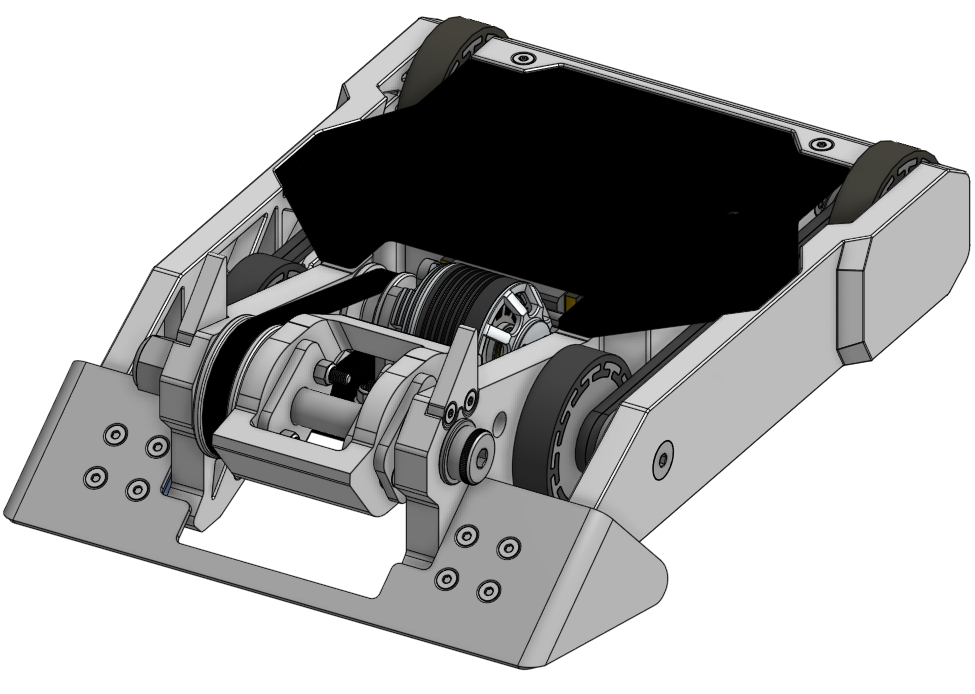
\includegraphics[scale=0.1]{very-original.png}
				\caption{Very Original}
				\label{Very Original}
			\end{minipage}
			\begin{minipage}{0.45\textwidth}
				\centering
				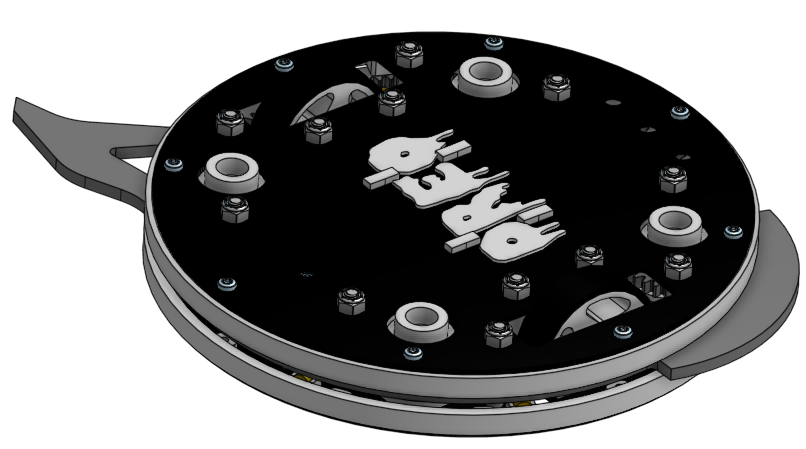
\includegraphics[scale=0.1]{double_stuffed.png}
				\caption{Double Stuffed}
				\label{Double Stuffed}
			\end{minipage}
		\end{figure}
	\item The Dynamic model will then be used in a Kinodynamic planner which will have the goal of hitting a moving opponent.
	\item A Oriented Bounding Box representing the opponent which will travel at a constant acceleration from a starting location and starting velocity.
	\item The robot will impact the side of the opponent while avoiding the opponent's front and back which will represent the opponent's weapons.
	\item The robot will not impact the opponent with any part of itself except for the weapon.
	\item The robot must avoid static and moving obstacles which will be represented as Oriented Bounding Boxes.
	\item The robot and its weapon will be represented by either Oriented Bounding Boxes or Circles.
	\item The generated motions must be visualized.
\end{itemize}

\section{Expected Challenges}
\begin{itemize}
	\item The force generated by accelerating a robot's weapon will likely be difficult to model.
	\item I have no experience in visualizing trajectories.
	\item Combat robots can be very different, and since this is meant to be generalized it will likely be difficult to model them for validity checking.
\end{itemize}




\end{document}